% !TEX encoding = UTF-8 Unicode
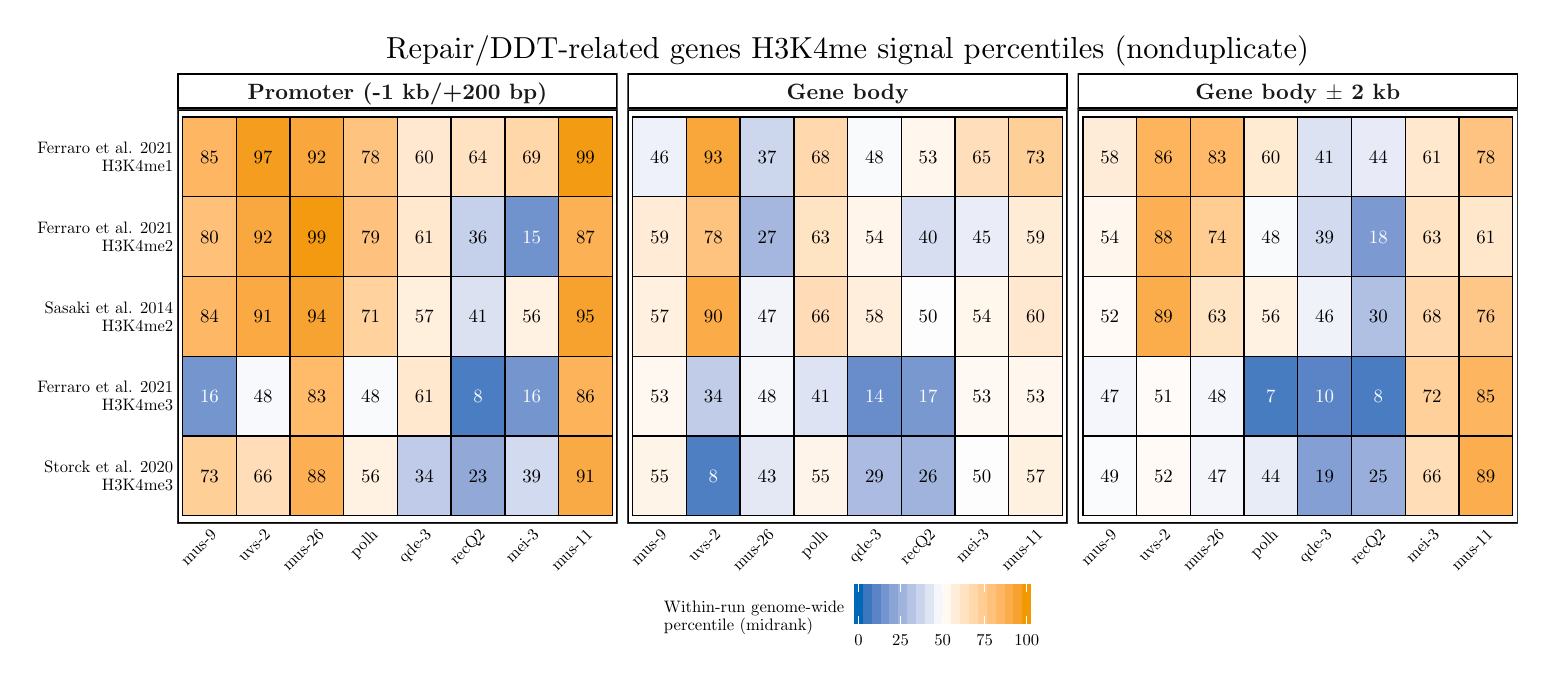
\begin{tikzpicture}[x=1pt,y=1pt]
\definecolor{fillColor}{RGB}{255,255,255}
\path[use as bounding box,fill=fillColor,fill opacity=0.00] (0,0) rectangle (542.02,231.26);
\begin{scope}
\path[clip] (  0.00,  0.00) rectangle (542.02,231.26);
\definecolor{drawColor}{RGB}{255,255,255}
\definecolor{fillColor}{RGB}{255,255,255}

\path[draw=drawColor,line width= 0.7pt,line join=round,line cap=round,fill=fillColor] ( -0.00,  0.00) rectangle (542.02,231.26);
\end{scope}
\begin{scope}
\path[clip] ( 54.02, 52.00) rectangle (213.19,201.87);
\definecolor{drawColor}{RGB}{0,0,0}
\definecolor{fillColor}{RGB}{255,255,255}

\path[draw=drawColor,line width= 1.1pt,line join=round,line cap=round,fill=fillColor] ( 54.02, 52.00) rectangle (213.19,201.87);
\definecolor{fillColor}{RGB}{254,182,98}

\path[draw=drawColor,line width= 0.5pt,fill=fillColor] ( 55.96,170.17) rectangle ( 75.37,198.99);
\definecolor{fillColor}{RGB}{245,157,30}

\path[draw=drawColor,line width= 0.5pt,fill=fillColor] ( 75.37,170.17) rectangle ( 94.78,198.99);
\definecolor{fillColor}{RGB}{249,167,61}

\path[draw=drawColor,line width= 0.5pt,fill=fillColor] ( 94.78,170.17) rectangle (114.19,198.99);
\definecolor{fillColor}{RGB}{255,195,128}

\path[draw=drawColor,line width= 0.5pt,fill=fillColor] (114.19,170.17) rectangle (133.61,198.99);
\definecolor{fillColor}{RGB}{255,232,207}

\path[draw=drawColor,line width= 0.5pt,fill=fillColor] (133.61,170.17) rectangle (153.02,198.99);
\definecolor{fillColor}{RGB}{255,226,193}

\path[draw=drawColor,line width= 0.5pt,fill=fillColor] (153.02,170.17) rectangle (172.43,198.99);
\definecolor{fillColor}{RGB}{255,215,169}

\path[draw=drawColor,line width= 0.5pt,fill=fillColor] (172.43,170.17) rectangle (191.84,198.99);
\definecolor{fillColor}{RGB}{243,155,19}

\path[draw=drawColor,line width= 0.5pt,fill=fillColor] (191.84,170.17) rectangle (211.25,198.99);
\definecolor{fillColor}{RGB}{255,192,121}

\path[draw=drawColor,line width= 0.5pt,fill=fillColor] ( 55.96,141.35) rectangle ( 75.37,170.17);
\definecolor{fillColor}{RGB}{249,168,63}

\path[draw=drawColor,line width= 0.5pt,fill=fillColor] ( 75.37,141.35) rectangle ( 94.78,170.17);
\definecolor{fillColor}{RGB}{243,154,16}

\path[draw=drawColor,line width= 0.5pt,fill=fillColor] ( 94.78,141.35) rectangle (114.19,170.17);
\definecolor{fillColor}{RGB}{255,194,126}

\path[draw=drawColor,line width= 0.5pt,fill=fillColor] (114.19,141.35) rectangle (133.61,170.17);
\definecolor{fillColor}{RGB}{255,232,205}

\path[draw=drawColor,line width= 0.5pt,fill=fillColor] (133.61,141.35) rectangle (153.02,170.17);
\definecolor{fillColor}{RGB}{197,208,234}

\path[draw=drawColor,line width= 0.5pt,fill=fillColor] (153.02,141.35) rectangle (172.43,170.17);
\definecolor{fillColor}{RGB}{113,147,205}

\path[draw=drawColor,line width= 0.5pt,fill=fillColor] (172.43,141.35) rectangle (191.84,170.17);
\definecolor{fillColor}{RGB}{252,177,85}

\path[draw=drawColor,line width= 0.5pt,fill=fillColor] (191.84,141.35) rectangle (211.25,170.17);
\definecolor{fillColor}{RGB}{254,183,100}

\path[draw=drawColor,line width= 0.5pt,fill=fillColor] ( 55.96,112.53) rectangle ( 75.37,141.35);
\definecolor{fillColor}{RGB}{250,169,67}

\path[draw=drawColor,line width= 0.5pt,fill=fillColor] ( 75.37,112.53) rectangle ( 94.78,141.35);
\definecolor{fillColor}{RGB}{247,163,50}

\path[draw=drawColor,line width= 0.5pt,fill=fillColor] ( 94.78,112.53) rectangle (114.19,141.35);
\definecolor{fillColor}{RGB}{255,210,158}

\path[draw=drawColor,line width= 0.5pt,fill=fillColor] (114.19,112.53) rectangle (133.61,141.35);
\definecolor{fillColor}{RGB}{255,239,221}

\path[draw=drawColor,line width= 0.5pt,fill=fillColor] (133.61,112.53) rectangle (153.02,141.35);
\definecolor{fillColor}{RGB}{219,225,241}

\path[draw=drawColor,line width= 0.5pt,fill=fillColor] (153.02,112.53) rectangle (172.43,141.35);
\definecolor{fillColor}{RGB}{255,242,227}

\path[draw=drawColor,line width= 0.5pt,fill=fillColor] (172.43,112.53) rectangle (191.84,141.35);
\definecolor{fillColor}{RGB}{247,162,47}

\path[draw=drawColor,line width= 0.5pt,fill=fillColor] (191.84,112.53) rectangle (211.25,141.35);
\definecolor{fillColor}{RGB}{116,149,206}

\path[draw=drawColor,line width= 0.5pt,fill=fillColor] ( 55.96, 83.71) rectangle ( 75.37,112.53);
\definecolor{fillColor}{RGB}{248,249,252}

\path[draw=drawColor,line width= 0.5pt,fill=fillColor] ( 75.37, 83.71) rectangle ( 94.78,112.53);
\definecolor{fillColor}{RGB}{255,186,106}

\path[draw=drawColor,line width= 0.5pt,fill=fillColor] ( 94.78, 83.71) rectangle (114.19,112.53);
\definecolor{fillColor}{RGB}{249,250,252}

\path[draw=drawColor,line width= 0.5pt,fill=fillColor] (114.19, 83.71) rectangle (133.61,112.53);
\definecolor{fillColor}{RGB}{255,232,206}

\path[draw=drawColor,line width= 0.5pt,fill=fillColor] (133.61, 83.71) rectangle (153.02,112.53);
\definecolor{fillColor}{RGB}{75,125,194}

\path[draw=drawColor,line width= 0.5pt,fill=fillColor] (153.02, 83.71) rectangle (172.43,112.53);
\definecolor{fillColor}{RGB}{117,149,206}

\path[draw=drawColor,line width= 0.5pt,fill=fillColor] (172.43, 83.71) rectangle (191.84,112.53);
\definecolor{fillColor}{RGB}{253,179,90}

\path[draw=drawColor,line width= 0.5pt,fill=fillColor] (191.84, 83.71) rectangle (211.25,112.53);
\definecolor{fillColor}{RGB}{255,207,152}

\path[draw=drawColor,line width= 0.5pt,fill=fillColor] ( 55.96, 54.88) rectangle ( 75.37, 83.71);
\definecolor{fillColor}{RGB}{255,221,184}

\path[draw=drawColor,line width= 0.5pt,fill=fillColor] ( 75.37, 54.88) rectangle ( 94.78, 83.71);
\definecolor{fillColor}{RGB}{252,176,83}

\path[draw=drawColor,line width= 0.5pt,fill=fillColor] ( 94.78, 54.88) rectangle (114.19, 83.71);
\definecolor{fillColor}{RGB}{255,242,227}

\path[draw=drawColor,line width= 0.5pt,fill=fillColor] (114.19, 54.88) rectangle (133.61, 83.71);
\definecolor{fillColor}{RGB}{191,203,232}

\path[draw=drawColor,line width= 0.5pt,fill=fillColor] (133.61, 54.88) rectangle (153.02, 83.71);
\definecolor{fillColor}{RGB}{146,169,216}

\path[draw=drawColor,line width= 0.5pt,fill=fillColor] (153.02, 54.88) rectangle (172.43, 83.71);
\definecolor{fillColor}{RGB}{209,218,238}

\path[draw=drawColor,line width= 0.5pt,fill=fillColor] (172.43, 54.88) rectangle (191.84, 83.71);
\definecolor{fillColor}{RGB}{250,170,68}

\path[draw=drawColor,line width= 0.5pt,fill=fillColor] (191.84, 54.88) rectangle (211.25, 83.71);

\node[text=drawColor,anchor=base,inner sep=0pt, outer sep=0pt, scale=  0.68] at ( 65.67,182.23) {85};

\node[text=drawColor,anchor=base,inner sep=0pt, outer sep=0pt, scale=  0.68] at ( 85.08,182.23) {97};

\node[text=drawColor,anchor=base,inner sep=0pt, outer sep=0pt, scale=  0.68] at (104.49,182.23) {92};

\node[text=drawColor,anchor=base,inner sep=0pt, outer sep=0pt, scale=  0.68] at (123.90,182.23) {78};

\node[text=drawColor,anchor=base,inner sep=0pt, outer sep=0pt, scale=  0.68] at (143.31,182.23) {60};

\node[text=drawColor,anchor=base,inner sep=0pt, outer sep=0pt, scale=  0.68] at (162.72,182.23) {64};

\node[text=drawColor,anchor=base,inner sep=0pt, outer sep=0pt, scale=  0.68] at (182.13,182.23) {69};

\node[text=drawColor,anchor=base,inner sep=0pt, outer sep=0pt, scale=  0.68] at (201.54,182.23) {99};

\node[text=drawColor,anchor=base,inner sep=0pt, outer sep=0pt, scale=  0.68] at ( 65.67,153.41) {80};

\node[text=drawColor,anchor=base,inner sep=0pt, outer sep=0pt, scale=  0.68] at ( 85.08,153.41) {92};

\node[text=drawColor,anchor=base,inner sep=0pt, outer sep=0pt, scale=  0.68] at (104.49,153.41) {99};

\node[text=drawColor,anchor=base,inner sep=0pt, outer sep=0pt, scale=  0.68] at (123.90,153.41) {79};

\node[text=drawColor,anchor=base,inner sep=0pt, outer sep=0pt, scale=  0.68] at (143.31,153.41) {61};

\node[text=drawColor,anchor=base,inner sep=0pt, outer sep=0pt, scale=  0.68] at (162.72,153.41) {36};
\definecolor{drawColor}{RGB}{255,255,255}

\node[text=drawColor,anchor=base,inner sep=0pt, outer sep=0pt, scale=  0.68] at (182.13,153.41) {15};
\definecolor{drawColor}{RGB}{0,0,0}

\node[text=drawColor,anchor=base,inner sep=0pt, outer sep=0pt, scale=  0.68] at (201.54,153.41) {87};

\node[text=drawColor,anchor=base,inner sep=0pt, outer sep=0pt, scale=  0.68] at ( 65.67,124.59) {84};

\node[text=drawColor,anchor=base,inner sep=0pt, outer sep=0pt, scale=  0.68] at ( 85.08,124.59) {91};

\node[text=drawColor,anchor=base,inner sep=0pt, outer sep=0pt, scale=  0.68] at (104.49,124.59) {94};

\node[text=drawColor,anchor=base,inner sep=0pt, outer sep=0pt, scale=  0.68] at (123.90,124.59) {71};

\node[text=drawColor,anchor=base,inner sep=0pt, outer sep=0pt, scale=  0.68] at (143.31,124.59) {57};

\node[text=drawColor,anchor=base,inner sep=0pt, outer sep=0pt, scale=  0.68] at (162.72,124.59) {41};

\node[text=drawColor,anchor=base,inner sep=0pt, outer sep=0pt, scale=  0.68] at (182.13,124.59) {56};

\node[text=drawColor,anchor=base,inner sep=0pt, outer sep=0pt, scale=  0.68] at (201.54,124.59) {95};
\definecolor{drawColor}{RGB}{255,255,255}

\node[text=drawColor,anchor=base,inner sep=0pt, outer sep=0pt, scale=  0.68] at ( 65.67, 95.76) {16};
\definecolor{drawColor}{RGB}{0,0,0}

\node[text=drawColor,anchor=base,inner sep=0pt, outer sep=0pt, scale=  0.68] at ( 85.08, 95.76) {48};

\node[text=drawColor,anchor=base,inner sep=0pt, outer sep=0pt, scale=  0.68] at (104.49, 95.76) {83};

\node[text=drawColor,anchor=base,inner sep=0pt, outer sep=0pt, scale=  0.68] at (123.90, 95.76) {48};

\node[text=drawColor,anchor=base,inner sep=0pt, outer sep=0pt, scale=  0.68] at (143.31, 95.76) {61};
\definecolor{drawColor}{RGB}{255,255,255}

\node[text=drawColor,anchor=base,inner sep=0pt, outer sep=0pt, scale=  0.68] at (162.72, 95.76) {8};

\node[text=drawColor,anchor=base,inner sep=0pt, outer sep=0pt, scale=  0.68] at (182.13, 95.76) {16};
\definecolor{drawColor}{RGB}{0,0,0}

\node[text=drawColor,anchor=base,inner sep=0pt, outer sep=0pt, scale=  0.68] at (201.54, 95.76) {86};

\node[text=drawColor,anchor=base,inner sep=0pt, outer sep=0pt, scale=  0.68] at ( 65.67, 66.94) {73};

\node[text=drawColor,anchor=base,inner sep=0pt, outer sep=0pt, scale=  0.68] at ( 85.08, 66.94) {66};

\node[text=drawColor,anchor=base,inner sep=0pt, outer sep=0pt, scale=  0.68] at (104.49, 66.94) {88};

\node[text=drawColor,anchor=base,inner sep=0pt, outer sep=0pt, scale=  0.68] at (123.90, 66.94) {56};

\node[text=drawColor,anchor=base,inner sep=0pt, outer sep=0pt, scale=  0.68] at (143.31, 66.94) {34};

\node[text=drawColor,anchor=base,inner sep=0pt, outer sep=0pt, scale=  0.68] at (162.72, 66.94) {23};

\node[text=drawColor,anchor=base,inner sep=0pt, outer sep=0pt, scale=  0.68] at (182.13, 66.94) {39};

\node[text=drawColor,anchor=base,inner sep=0pt, outer sep=0pt, scale=  0.68] at (201.54, 66.94) {91};
\definecolor{drawColor}{gray}{0.20}

\path[draw=drawColor,line width= 0.7pt,line join=round,line cap=round] ( 54.02, 52.00) rectangle (213.19,201.87);
\end{scope}
\begin{scope}
\path[clip] (216.69, 52.00) rectangle (375.86,201.87);
\definecolor{drawColor}{RGB}{0,0,0}
\definecolor{fillColor}{RGB}{255,255,255}

\path[draw=drawColor,line width= 1.1pt,line join=round,line cap=round,fill=fillColor] (216.69, 52.00) rectangle (375.86,201.87);
\definecolor{fillColor}{RGB}{238,241,249}

\path[draw=drawColor,line width= 0.5pt,fill=fillColor] (218.63,170.17) rectangle (238.04,198.99);
\definecolor{fillColor}{RGB}{249,166,58}

\path[draw=drawColor,line width= 0.5pt,fill=fillColor] (238.04,170.17) rectangle (257.45,198.99);
\definecolor{fillColor}{RGB}{204,214,237}

\path[draw=drawColor,line width= 0.5pt,fill=fillColor] (257.45,170.17) rectangle (276.86,198.99);
\definecolor{fillColor}{RGB}{255,217,173}

\path[draw=drawColor,line width= 0.5pt,fill=fillColor] (276.86,170.17) rectangle (296.27,198.99);
\definecolor{fillColor}{RGB}{249,250,252}

\path[draw=drawColor,line width= 0.5pt,fill=fillColor] (296.27,170.17) rectangle (315.68,198.99);
\definecolor{fillColor}{RGB}{255,247,238}

\path[draw=drawColor,line width= 0.5pt,fill=fillColor] (315.68,170.17) rectangle (335.09,198.99);
\definecolor{fillColor}{RGB}{255,223,187}

\path[draw=drawColor,line width= 0.5pt,fill=fillColor] (335.09,170.17) rectangle (354.51,198.99);
\definecolor{fillColor}{RGB}{255,207,152}

\path[draw=drawColor,line width= 0.5pt,fill=fillColor] (354.51,170.17) rectangle (373.92,198.99);
\definecolor{fillColor}{RGB}{255,235,214}

\path[draw=drawColor,line width= 0.5pt,fill=fillColor] (218.63,141.35) rectangle (238.04,170.17);
\definecolor{fillColor}{RGB}{255,195,128}

\path[draw=drawColor,line width= 0.5pt,fill=fillColor] (238.04,141.35) rectangle (257.45,170.17);
\definecolor{fillColor}{RGB}{165,183,222}

\path[draw=drawColor,line width= 0.5pt,fill=fillColor] (257.45,141.35) rectangle (276.86,170.17);
\definecolor{fillColor}{RGB}{255,228,196}

\path[draw=drawColor,line width= 0.5pt,fill=fillColor] (276.86,141.35) rectangle (296.27,170.17);
\definecolor{fillColor}{RGB}{255,245,235}

\path[draw=drawColor,line width= 0.5pt,fill=fillColor] (296.27,141.35) rectangle (315.68,170.17);
\definecolor{fillColor}{RGB}{215,222,241}

\path[draw=drawColor,line width= 0.5pt,fill=fillColor] (315.68,141.35) rectangle (335.09,170.17);
\definecolor{fillColor}{RGB}{234,237,247}

\path[draw=drawColor,line width= 0.5pt,fill=fillColor] (335.09,141.35) rectangle (354.51,170.17);
\definecolor{fillColor}{RGB}{255,236,214}

\path[draw=drawColor,line width= 0.5pt,fill=fillColor] (354.51,141.35) rectangle (373.92,170.17);
\definecolor{fillColor}{RGB}{255,240,223}

\path[draw=drawColor,line width= 0.5pt,fill=fillColor] (218.63,112.53) rectangle (238.04,141.35);
\definecolor{fillColor}{RGB}{251,172,73}

\path[draw=drawColor,line width= 0.5pt,fill=fillColor] (238.04,112.53) rectangle (257.45,141.35);
\definecolor{fillColor}{RGB}{242,244,250}

\path[draw=drawColor,line width= 0.5pt,fill=fillColor] (257.45,112.53) rectangle (276.86,141.35);
\definecolor{fillColor}{RGB}{255,220,183}

\path[draw=drawColor,line width= 0.5pt,fill=fillColor] (276.86,112.53) rectangle (296.27,141.35);
\definecolor{fillColor}{RGB}{255,238,219}

\path[draw=drawColor,line width= 0.5pt,fill=fillColor] (296.27,112.53) rectangle (315.68,141.35);
\definecolor{fillColor}{RGB}{254,253,253}

\path[draw=drawColor,line width= 0.5pt,fill=fillColor] (315.68,112.53) rectangle (335.09,141.35);
\definecolor{fillColor}{RGB}{255,246,236}

\path[draw=drawColor,line width= 0.5pt,fill=fillColor] (335.09,112.53) rectangle (354.51,141.35);
\definecolor{fillColor}{RGB}{255,232,207}

\path[draw=drawColor,line width= 0.5pt,fill=fillColor] (354.51,112.53) rectangle (373.92,141.35);
\definecolor{fillColor}{RGB}{255,248,240}

\path[draw=drawColor,line width= 0.5pt,fill=fillColor] (218.63, 83.71) rectangle (238.04,112.53);
\definecolor{fillColor}{RGB}{192,204,232}

\path[draw=drawColor,line width= 0.5pt,fill=fillColor] (238.04, 83.71) rectangle (257.45,112.53);
\definecolor{fillColor}{RGB}{246,247,251}

\path[draw=drawColor,line width= 0.5pt,fill=fillColor] (257.45, 83.71) rectangle (276.86,112.53);
\definecolor{fillColor}{RGB}{221,227,242}

\path[draw=drawColor,line width= 0.5pt,fill=fillColor] (276.86, 83.71) rectangle (296.27,112.53);
\definecolor{fillColor}{RGB}{105,141,202}

\path[draw=drawColor,line width= 0.5pt,fill=fillColor] (296.27, 83.71) rectangle (315.68,112.53);
\definecolor{fillColor}{RGB}{121,152,208}

\path[draw=drawColor,line width= 0.5pt,fill=fillColor] (315.68, 83.71) rectangle (335.09,112.53);
\definecolor{fillColor}{RGB}{255,249,243}

\path[draw=drawColor,line width= 0.5pt,fill=fillColor] (335.09, 83.71) rectangle (354.51,112.53);
\definecolor{fillColor}{RGB}{255,247,238}

\path[draw=drawColor,line width= 0.5pt,fill=fillColor] (354.51, 83.71) rectangle (373.92,112.53);
\definecolor{fillColor}{RGB}{255,244,232}

\path[draw=drawColor,line width= 0.5pt,fill=fillColor] (218.63, 54.88) rectangle (238.04, 83.71);
\definecolor{fillColor}{RGB}{78,127,195}

\path[draw=drawColor,line width= 0.5pt,fill=fillColor] (238.04, 54.88) rectangle (257.45, 83.71);
\definecolor{fillColor}{RGB}{228,232,245}

\path[draw=drawColor,line width= 0.5pt,fill=fillColor] (257.45, 54.88) rectangle (276.86, 83.71);
\definecolor{fillColor}{RGB}{255,244,233}

\path[draw=drawColor,line width= 0.5pt,fill=fillColor] (276.86, 54.88) rectangle (296.27, 83.71);
\definecolor{fillColor}{RGB}{171,187,225}

\path[draw=drawColor,line width= 0.5pt,fill=fillColor] (296.27, 54.88) rectangle (315.68, 83.71);
\definecolor{fillColor}{RGB}{160,179,221}

\path[draw=drawColor,line width= 0.5pt,fill=fillColor] (315.68, 54.88) rectangle (335.09, 83.71);
\definecolor{fillColor}{RGB}{254,253,253}

\path[draw=drawColor,line width= 0.5pt,fill=fillColor] (335.09, 54.88) rectangle (354.51, 83.71);
\definecolor{fillColor}{RGB}{255,241,224}

\path[draw=drawColor,line width= 0.5pt,fill=fillColor] (354.51, 54.88) rectangle (373.92, 83.71);

\node[text=drawColor,anchor=base,inner sep=0pt, outer sep=0pt, scale=  0.68] at (228.34,182.23) {46};

\node[text=drawColor,anchor=base,inner sep=0pt, outer sep=0pt, scale=  0.68] at (247.75,182.23) {93};

\node[text=drawColor,anchor=base,inner sep=0pt, outer sep=0pt, scale=  0.68] at (267.16,182.23) {37};

\node[text=drawColor,anchor=base,inner sep=0pt, outer sep=0pt, scale=  0.68] at (286.57,182.23) {68};

\node[text=drawColor,anchor=base,inner sep=0pt, outer sep=0pt, scale=  0.68] at (305.98,182.23) {48};

\node[text=drawColor,anchor=base,inner sep=0pt, outer sep=0pt, scale=  0.68] at (325.39,182.23) {53};

\node[text=drawColor,anchor=base,inner sep=0pt, outer sep=0pt, scale=  0.68] at (344.80,182.23) {65};

\node[text=drawColor,anchor=base,inner sep=0pt, outer sep=0pt, scale=  0.68] at (364.21,182.23) {73};

\node[text=drawColor,anchor=base,inner sep=0pt, outer sep=0pt, scale=  0.68] at (228.34,153.41) {59};

\node[text=drawColor,anchor=base,inner sep=0pt, outer sep=0pt, scale=  0.68] at (247.75,153.41) {78};

\node[text=drawColor,anchor=base,inner sep=0pt, outer sep=0pt, scale=  0.68] at (267.16,153.41) {27};

\node[text=drawColor,anchor=base,inner sep=0pt, outer sep=0pt, scale=  0.68] at (286.57,153.41) {63};

\node[text=drawColor,anchor=base,inner sep=0pt, outer sep=0pt, scale=  0.68] at (305.98,153.41) {54};

\node[text=drawColor,anchor=base,inner sep=0pt, outer sep=0pt, scale=  0.68] at (325.39,153.41) {40};

\node[text=drawColor,anchor=base,inner sep=0pt, outer sep=0pt, scale=  0.68] at (344.80,153.41) {45};

\node[text=drawColor,anchor=base,inner sep=0pt, outer sep=0pt, scale=  0.68] at (364.21,153.41) {59};

\node[text=drawColor,anchor=base,inner sep=0pt, outer sep=0pt, scale=  0.68] at (228.34,124.59) {57};

\node[text=drawColor,anchor=base,inner sep=0pt, outer sep=0pt, scale=  0.68] at (247.75,124.59) {90};

\node[text=drawColor,anchor=base,inner sep=0pt, outer sep=0pt, scale=  0.68] at (267.16,124.59) {47};

\node[text=drawColor,anchor=base,inner sep=0pt, outer sep=0pt, scale=  0.68] at (286.57,124.59) {66};

\node[text=drawColor,anchor=base,inner sep=0pt, outer sep=0pt, scale=  0.68] at (305.98,124.59) {58};

\node[text=drawColor,anchor=base,inner sep=0pt, outer sep=0pt, scale=  0.68] at (325.39,124.59) {50};

\node[text=drawColor,anchor=base,inner sep=0pt, outer sep=0pt, scale=  0.68] at (344.80,124.59) {54};

\node[text=drawColor,anchor=base,inner sep=0pt, outer sep=0pt, scale=  0.68] at (364.21,124.59) {60};

\node[text=drawColor,anchor=base,inner sep=0pt, outer sep=0pt, scale=  0.68] at (228.34, 95.76) {53};

\node[text=drawColor,anchor=base,inner sep=0pt, outer sep=0pt, scale=  0.68] at (247.75, 95.76) {34};

\node[text=drawColor,anchor=base,inner sep=0pt, outer sep=0pt, scale=  0.68] at (267.16, 95.76) {48};

\node[text=drawColor,anchor=base,inner sep=0pt, outer sep=0pt, scale=  0.68] at (286.57, 95.76) {41};
\definecolor{drawColor}{RGB}{255,255,255}

\node[text=drawColor,anchor=base,inner sep=0pt, outer sep=0pt, scale=  0.68] at (305.98, 95.76) {14};

\node[text=drawColor,anchor=base,inner sep=0pt, outer sep=0pt, scale=  0.68] at (325.39, 95.76) {17};
\definecolor{drawColor}{RGB}{0,0,0}

\node[text=drawColor,anchor=base,inner sep=0pt, outer sep=0pt, scale=  0.68] at (344.80, 95.76) {53};

\node[text=drawColor,anchor=base,inner sep=0pt, outer sep=0pt, scale=  0.68] at (364.21, 95.76) {53};

\node[text=drawColor,anchor=base,inner sep=0pt, outer sep=0pt, scale=  0.68] at (228.34, 66.94) {55};
\definecolor{drawColor}{RGB}{255,255,255}

\node[text=drawColor,anchor=base,inner sep=0pt, outer sep=0pt, scale=  0.68] at (247.75, 66.94) {8};
\definecolor{drawColor}{RGB}{0,0,0}

\node[text=drawColor,anchor=base,inner sep=0pt, outer sep=0pt, scale=  0.68] at (267.16, 66.94) {43};

\node[text=drawColor,anchor=base,inner sep=0pt, outer sep=0pt, scale=  0.68] at (286.57, 66.94) {55};

\node[text=drawColor,anchor=base,inner sep=0pt, outer sep=0pt, scale=  0.68] at (305.98, 66.94) {29};

\node[text=drawColor,anchor=base,inner sep=0pt, outer sep=0pt, scale=  0.68] at (325.39, 66.94) {26};

\node[text=drawColor,anchor=base,inner sep=0pt, outer sep=0pt, scale=  0.68] at (344.80, 66.94) {50};

\node[text=drawColor,anchor=base,inner sep=0pt, outer sep=0pt, scale=  0.68] at (364.21, 66.94) {57};
\definecolor{drawColor}{gray}{0.20}

\path[draw=drawColor,line width= 0.7pt,line join=round,line cap=round] (216.69, 52.00) rectangle (375.86,201.87);
\end{scope}
\begin{scope}
\path[clip] (379.36, 52.00) rectangle (538.52,201.87);
\definecolor{drawColor}{RGB}{0,0,0}
\definecolor{fillColor}{RGB}{255,255,255}

\path[draw=drawColor,line width= 1.1pt,line join=round,line cap=round,fill=fillColor] (379.36, 52.00) rectangle (538.53,201.87);
\definecolor{fillColor}{RGB}{255,236,216}

\path[draw=drawColor,line width= 0.5pt,fill=fillColor] (381.30,170.17) rectangle (400.71,198.99);
\definecolor{fillColor}{RGB}{254,180,93}

\path[draw=drawColor,line width= 0.5pt,fill=fillColor] (400.71,170.17) rectangle (420.12,198.99);
\definecolor{fillColor}{RGB}{255,185,104}

\path[draw=drawColor,line width= 0.5pt,fill=fillColor] (420.12,170.17) rectangle (439.53,198.99);
\definecolor{fillColor}{RGB}{255,234,210}

\path[draw=drawColor,line width= 0.5pt,fill=fillColor] (439.53,170.17) rectangle (458.94,198.99);
\definecolor{fillColor}{RGB}{220,226,242}

\path[draw=drawColor,line width= 0.5pt,fill=fillColor] (458.94,170.17) rectangle (478.35,198.99);
\definecolor{fillColor}{RGB}{232,235,247}

\path[draw=drawColor,line width= 0.5pt,fill=fillColor] (478.35,170.17) rectangle (497.76,198.99);
\definecolor{fillColor}{RGB}{255,232,206}

\path[draw=drawColor,line width= 0.5pt,fill=fillColor] (497.76,170.17) rectangle (517.17,198.99);
\definecolor{fillColor}{RGB}{255,195,129}

\path[draw=drawColor,line width= 0.5pt,fill=fillColor] (517.17,170.17) rectangle (536.58,198.99);
\definecolor{fillColor}{RGB}{255,246,237}

\path[draw=drawColor,line width= 0.5pt,fill=fillColor] (381.30,141.35) rectangle (400.71,170.17);
\definecolor{fillColor}{RGB}{252,176,83}

\path[draw=drawColor,line width= 0.5pt,fill=fillColor] (400.71,141.35) rectangle (420.12,170.17);
\definecolor{fillColor}{RGB}{255,204,146}

\path[draw=drawColor,line width= 0.5pt,fill=fillColor] (420.12,141.35) rectangle (439.53,170.17);
\definecolor{fillColor}{RGB}{249,250,252}

\path[draw=drawColor,line width= 0.5pt,fill=fillColor] (439.53,141.35) rectangle (458.94,170.17);
\definecolor{fillColor}{RGB}{209,218,239}

\path[draw=drawColor,line width= 0.5pt,fill=fillColor] (458.94,141.35) rectangle (478.35,170.17);
\definecolor{fillColor}{RGB}{124,154,209}

\path[draw=drawColor,line width= 0.5pt,fill=fillColor] (478.35,141.35) rectangle (497.76,170.17);
\definecolor{fillColor}{RGB}{255,227,194}

\path[draw=drawColor,line width= 0.5pt,fill=fillColor] (497.76,141.35) rectangle (517.17,170.17);
\definecolor{fillColor}{RGB}{255,231,204}

\path[draw=drawColor,line width= 0.5pt,fill=fillColor] (517.17,141.35) rectangle (536.58,170.17);
\definecolor{fillColor}{RGB}{255,250,246}

\path[draw=drawColor,line width= 0.5pt,fill=fillColor] (381.30,112.53) rectangle (400.71,141.35);
\definecolor{fillColor}{RGB}{251,173,76}

\path[draw=drawColor,line width= 0.5pt,fill=fillColor] (400.71,112.53) rectangle (420.12,141.35);
\definecolor{fillColor}{RGB}{255,228,196}

\path[draw=drawColor,line width= 0.5pt,fill=fillColor] (420.12,112.53) rectangle (439.53,141.35);
\definecolor{fillColor}{RGB}{255,242,226}

\path[draw=drawColor,line width= 0.5pt,fill=fillColor] (439.53,112.53) rectangle (458.94,141.35);
\definecolor{fillColor}{RGB}{240,242,250}

\path[draw=drawColor,line width= 0.5pt,fill=fillColor] (458.94,112.53) rectangle (478.35,141.35);
\definecolor{fillColor}{RGB}{176,192,227}

\path[draw=drawColor,line width= 0.5pt,fill=fillColor] (478.35,112.53) rectangle (497.76,141.35);
\definecolor{fillColor}{RGB}{255,217,173}

\path[draw=drawColor,line width= 0.5pt,fill=fillColor] (497.76,112.53) rectangle (517.17,141.35);
\definecolor{fillColor}{RGB}{255,199,135}

\path[draw=drawColor,line width= 0.5pt,fill=fillColor] (517.17,112.53) rectangle (536.58,141.35);
\definecolor{fillColor}{RGB}{245,246,251}

\path[draw=drawColor,line width= 0.5pt,fill=fillColor] (381.30, 83.71) rectangle (400.71,112.53);
\definecolor{fillColor}{RGB}{255,251,248}

\path[draw=drawColor,line width= 0.5pt,fill=fillColor] (400.71, 83.71) rectangle (420.12,112.53);
\definecolor{fillColor}{RGB}{245,246,251}

\path[draw=drawColor,line width= 0.5pt,fill=fillColor] (420.12, 83.71) rectangle (439.53,112.53);
\definecolor{fillColor}{RGB}{72,124,193}

\path[draw=drawColor,line width= 0.5pt,fill=fillColor] (439.53, 83.71) rectangle (458.94,112.53);
\definecolor{fillColor}{RGB}{90,132,198}

\path[draw=drawColor,line width= 0.5pt,fill=fillColor] (458.94, 83.71) rectangle (478.35,112.53);
\definecolor{fillColor}{RGB}{74,124,193}

\path[draw=drawColor,line width= 0.5pt,fill=fillColor] (478.35, 83.71) rectangle (497.76,112.53);
\definecolor{fillColor}{RGB}{255,208,154}

\path[draw=drawColor,line width= 0.5pt,fill=fillColor] (497.76, 83.71) rectangle (517.17,112.53);
\definecolor{fillColor}{RGB}{254,181,96}

\path[draw=drawColor,line width= 0.5pt,fill=fillColor] (517.17, 83.71) rectangle (536.58,112.53);
\definecolor{fillColor}{RGB}{250,251,252}

\path[draw=drawColor,line width= 0.5pt,fill=fillColor] (381.30, 54.88) rectangle (400.71, 83.71);
\definecolor{fillColor}{RGB}{255,250,245}

\path[draw=drawColor,line width= 0.5pt,fill=fillColor] (400.71, 54.88) rectangle (420.12, 83.71);
\definecolor{fillColor}{RGB}{243,245,251}

\path[draw=drawColor,line width= 0.5pt,fill=fillColor] (420.12, 54.88) rectangle (439.53, 83.71);
\definecolor{fillColor}{RGB}{232,236,247}

\path[draw=drawColor,line width= 0.5pt,fill=fillColor] (439.53, 54.88) rectangle (458.94, 83.71);
\definecolor{fillColor}{RGB}{131,159,211}

\path[draw=drawColor,line width= 0.5pt,fill=fillColor] (458.94, 54.88) rectangle (478.35, 83.71);
\definecolor{fillColor}{RGB}{153,174,218}

\path[draw=drawColor,line width= 0.5pt,fill=fillColor] (478.35, 54.88) rectangle (497.76, 83.71);
\definecolor{fillColor}{RGB}{255,221,183}

\path[draw=drawColor,line width= 0.5pt,fill=fillColor] (497.76, 54.88) rectangle (517.17, 83.71);
\definecolor{fillColor}{RGB}{252,174,79}

\path[draw=drawColor,line width= 0.5pt,fill=fillColor] (517.17, 54.88) rectangle (536.58, 83.71);

\node[text=drawColor,anchor=base,inner sep=0pt, outer sep=0pt, scale=  0.68] at (391.00,182.23) {58};

\node[text=drawColor,anchor=base,inner sep=0pt, outer sep=0pt, scale=  0.68] at (410.41,182.23) {86};

\node[text=drawColor,anchor=base,inner sep=0pt, outer sep=0pt, scale=  0.68] at (429.83,182.23) {83};

\node[text=drawColor,anchor=base,inner sep=0pt, outer sep=0pt, scale=  0.68] at (449.24,182.23) {60};

\node[text=drawColor,anchor=base,inner sep=0pt, outer sep=0pt, scale=  0.68] at (468.65,182.23) {41};

\node[text=drawColor,anchor=base,inner sep=0pt, outer sep=0pt, scale=  0.68] at (488.06,182.23) {44};

\node[text=drawColor,anchor=base,inner sep=0pt, outer sep=0pt, scale=  0.68] at (507.47,182.23) {61};

\node[text=drawColor,anchor=base,inner sep=0pt, outer sep=0pt, scale=  0.68] at (526.88,182.23) {78};

\node[text=drawColor,anchor=base,inner sep=0pt, outer sep=0pt, scale=  0.68] at (391.00,153.41) {54};

\node[text=drawColor,anchor=base,inner sep=0pt, outer sep=0pt, scale=  0.68] at (410.41,153.41) {88};

\node[text=drawColor,anchor=base,inner sep=0pt, outer sep=0pt, scale=  0.68] at (429.83,153.41) {74};

\node[text=drawColor,anchor=base,inner sep=0pt, outer sep=0pt, scale=  0.68] at (449.24,153.41) {48};

\node[text=drawColor,anchor=base,inner sep=0pt, outer sep=0pt, scale=  0.68] at (468.65,153.41) {39};
\definecolor{drawColor}{RGB}{255,255,255}

\node[text=drawColor,anchor=base,inner sep=0pt, outer sep=0pt, scale=  0.68] at (488.06,153.41) {18};
\definecolor{drawColor}{RGB}{0,0,0}

\node[text=drawColor,anchor=base,inner sep=0pt, outer sep=0pt, scale=  0.68] at (507.47,153.41) {63};

\node[text=drawColor,anchor=base,inner sep=0pt, outer sep=0pt, scale=  0.68] at (526.88,153.41) {61};

\node[text=drawColor,anchor=base,inner sep=0pt, outer sep=0pt, scale=  0.68] at (391.00,124.59) {52};

\node[text=drawColor,anchor=base,inner sep=0pt, outer sep=0pt, scale=  0.68] at (410.41,124.59) {89};

\node[text=drawColor,anchor=base,inner sep=0pt, outer sep=0pt, scale=  0.68] at (429.83,124.59) {63};

\node[text=drawColor,anchor=base,inner sep=0pt, outer sep=0pt, scale=  0.68] at (449.24,124.59) {56};

\node[text=drawColor,anchor=base,inner sep=0pt, outer sep=0pt, scale=  0.68] at (468.65,124.59) {46};

\node[text=drawColor,anchor=base,inner sep=0pt, outer sep=0pt, scale=  0.68] at (488.06,124.59) {30};

\node[text=drawColor,anchor=base,inner sep=0pt, outer sep=0pt, scale=  0.68] at (507.47,124.59) {68};

\node[text=drawColor,anchor=base,inner sep=0pt, outer sep=0pt, scale=  0.68] at (526.88,124.59) {76};

\node[text=drawColor,anchor=base,inner sep=0pt, outer sep=0pt, scale=  0.68] at (391.00, 95.76) {47};

\node[text=drawColor,anchor=base,inner sep=0pt, outer sep=0pt, scale=  0.68] at (410.41, 95.76) {51};

\node[text=drawColor,anchor=base,inner sep=0pt, outer sep=0pt, scale=  0.68] at (429.83, 95.76) {48};
\definecolor{drawColor}{RGB}{255,255,255}

\node[text=drawColor,anchor=base,inner sep=0pt, outer sep=0pt, scale=  0.68] at (449.24, 95.76) {7};

\node[text=drawColor,anchor=base,inner sep=0pt, outer sep=0pt, scale=  0.68] at (468.65, 95.76) {10};

\node[text=drawColor,anchor=base,inner sep=0pt, outer sep=0pt, scale=  0.68] at (488.06, 95.76) {8};
\definecolor{drawColor}{RGB}{0,0,0}

\node[text=drawColor,anchor=base,inner sep=0pt, outer sep=0pt, scale=  0.68] at (507.47, 95.76) {72};

\node[text=drawColor,anchor=base,inner sep=0pt, outer sep=0pt, scale=  0.68] at (526.88, 95.76) {85};

\node[text=drawColor,anchor=base,inner sep=0pt, outer sep=0pt, scale=  0.68] at (391.00, 66.94) {49};

\node[text=drawColor,anchor=base,inner sep=0pt, outer sep=0pt, scale=  0.68] at (410.41, 66.94) {52};

\node[text=drawColor,anchor=base,inner sep=0pt, outer sep=0pt, scale=  0.68] at (429.83, 66.94) {47};

\node[text=drawColor,anchor=base,inner sep=0pt, outer sep=0pt, scale=  0.68] at (449.24, 66.94) {44};

\node[text=drawColor,anchor=base,inner sep=0pt, outer sep=0pt, scale=  0.68] at (468.65, 66.94) {19};

\node[text=drawColor,anchor=base,inner sep=0pt, outer sep=0pt, scale=  0.68] at (488.06, 66.94) {25};

\node[text=drawColor,anchor=base,inner sep=0pt, outer sep=0pt, scale=  0.68] at (507.47, 66.94) {66};

\node[text=drawColor,anchor=base,inner sep=0pt, outer sep=0pt, scale=  0.68] at (526.88, 66.94) {89};
\definecolor{drawColor}{gray}{0.20}

\path[draw=drawColor,line width= 0.7pt,line join=round,line cap=round] (379.36, 52.00) rectangle (538.53,201.87);
\end{scope}
\begin{scope}
\path[clip] ( 54.02,201.87) rectangle (213.19,214.55);
\definecolor{drawColor}{RGB}{0,0,0}
\definecolor{fillColor}{RGB}{255,255,255}

\path[draw=drawColor,line width= 1.1pt,line join=round,line cap=round,fill=fillColor] ( 54.02,201.87) rectangle (213.19,214.55);
\definecolor{drawColor}{gray}{0.10}

\node[text=drawColor,anchor=base,inner sep=0pt, outer sep=0pt, scale=  0.80] at (133.61,205.45) {\bfseries Promoter (-1 kb/+200 bp)};
\end{scope}
\begin{scope}
\path[clip] (216.69,201.87) rectangle (375.86,214.55);
\definecolor{drawColor}{RGB}{0,0,0}
\definecolor{fillColor}{RGB}{255,255,255}

\path[draw=drawColor,line width= 1.1pt,line join=round,line cap=round,fill=fillColor] (216.69,201.87) rectangle (375.86,214.55);
\definecolor{drawColor}{gray}{0.10}

\node[text=drawColor,anchor=base,inner sep=0pt, outer sep=0pt, scale=  0.80] at (296.27,205.45) {\bfseries Gene body};
\end{scope}
\begin{scope}
\path[clip] (379.36,201.87) rectangle (538.52,214.55);
\definecolor{drawColor}{RGB}{0,0,0}
\definecolor{fillColor}{RGB}{255,255,255}

\path[draw=drawColor,line width= 1.1pt,line join=round,line cap=round,fill=fillColor] (379.36,201.87) rectangle (538.53,214.55);
\definecolor{drawColor}{gray}{0.10}

\node[text=drawColor,anchor=base,inner sep=0pt, outer sep=0pt, scale=  0.80] at (458.94,205.45) {\bfseries Gene body $\pm$ 2 kb};
\end{scope}
\begin{scope}
\path[clip] (  0.00,  0.00) rectangle (542.02,231.26);
\definecolor{drawColor}{RGB}{0,0,0}

\node[text=drawColor,rotate= 45.00,anchor=base east,inner sep=0pt, outer sep=0pt, scale=  0.60] at ( 68.59, 47.68) {mus-9};

\node[text=drawColor,rotate= 45.00,anchor=base east,inner sep=0pt, outer sep=0pt, scale=  0.60] at ( 88.00, 47.68) {uvs-2};

\node[text=drawColor,rotate= 45.00,anchor=base east,inner sep=0pt, outer sep=0pt, scale=  0.60] at (107.41, 47.68) {mus-26};

\node[text=drawColor,rotate= 45.00,anchor=base east,inner sep=0pt, outer sep=0pt, scale=  0.60] at (126.82, 47.68) {polh};

\node[text=drawColor,rotate= 45.00,anchor=base east,inner sep=0pt, outer sep=0pt, scale=  0.60] at (146.23, 47.68) {qde-3};

\node[text=drawColor,rotate= 45.00,anchor=base east,inner sep=0pt, outer sep=0pt, scale=  0.60] at (165.64, 47.68) {recQ2};

\node[text=drawColor,rotate= 45.00,anchor=base east,inner sep=0pt, outer sep=0pt, scale=  0.60] at (185.05, 47.68) {mei-3};

\node[text=drawColor,rotate= 45.00,anchor=base east,inner sep=0pt, outer sep=0pt, scale=  0.60] at (204.47, 47.68) {mus-11};
\end{scope}
\begin{scope}
\path[clip] (  0.00,  0.00) rectangle (542.02,231.26);
\definecolor{drawColor}{RGB}{0,0,0}

\node[text=drawColor,rotate= 45.00,anchor=base east,inner sep=0pt, outer sep=0pt, scale=  0.60] at (231.26, 47.68) {mus-9};

\node[text=drawColor,rotate= 45.00,anchor=base east,inner sep=0pt, outer sep=0pt, scale=  0.60] at (250.67, 47.68) {uvs-2};

\node[text=drawColor,rotate= 45.00,anchor=base east,inner sep=0pt, outer sep=0pt, scale=  0.60] at (270.08, 47.68) {mus-26};

\node[text=drawColor,rotate= 45.00,anchor=base east,inner sep=0pt, outer sep=0pt, scale=  0.60] at (289.49, 47.68) {polh};

\node[text=drawColor,rotate= 45.00,anchor=base east,inner sep=0pt, outer sep=0pt, scale=  0.60] at (308.90, 47.68) {qde-3};

\node[text=drawColor,rotate= 45.00,anchor=base east,inner sep=0pt, outer sep=0pt, scale=  0.60] at (328.31, 47.68) {recQ2};

\node[text=drawColor,rotate= 45.00,anchor=base east,inner sep=0pt, outer sep=0pt, scale=  0.60] at (347.72, 47.68) {mei-3};

\node[text=drawColor,rotate= 45.00,anchor=base east,inner sep=0pt, outer sep=0pt, scale=  0.60] at (367.13, 47.68) {mus-11};
\end{scope}
\begin{scope}
\path[clip] (  0.00,  0.00) rectangle (542.02,231.26);
\definecolor{drawColor}{RGB}{0,0,0}

\node[text=drawColor,rotate= 45.00,anchor=base east,inner sep=0pt, outer sep=0pt, scale=  0.60] at (393.93, 47.68) {mus-9};

\node[text=drawColor,rotate= 45.00,anchor=base east,inner sep=0pt, outer sep=0pt, scale=  0.60] at (413.34, 47.68) {uvs-2};

\node[text=drawColor,rotate= 45.00,anchor=base east,inner sep=0pt, outer sep=0pt, scale=  0.60] at (432.75, 47.68) {mus-26};

\node[text=drawColor,rotate= 45.00,anchor=base east,inner sep=0pt, outer sep=0pt, scale=  0.60] at (452.16, 47.68) {polh};

\node[text=drawColor,rotate= 45.00,anchor=base east,inner sep=0pt, outer sep=0pt, scale=  0.60] at (471.57, 47.68) {qde-3};

\node[text=drawColor,rotate= 45.00,anchor=base east,inner sep=0pt, outer sep=0pt, scale=  0.60] at (490.98, 47.68) {recQ2};

\node[text=drawColor,rotate= 45.00,anchor=base east,inner sep=0pt, outer sep=0pt, scale=  0.60] at (510.39, 47.68) {mei-3};

\node[text=drawColor,rotate= 45.00,anchor=base east,inner sep=0pt, outer sep=0pt, scale=  0.60] at (529.80, 47.68) {mus-11};
\end{scope}
\begin{scope}
\path[clip] (  0.00,  0.00) rectangle (542.02,231.26);
\definecolor{drawColor}{RGB}{0,0,0}

\node[text=drawColor,anchor=base east,inner sep=0pt, outer sep=0pt, scale=  0.60] at ( 52.62, 70.47) {Storck et al. 2020};

\node[text=drawColor,anchor=base east,inner sep=0pt, outer sep=0pt, scale=  0.60] at ( 52.62, 63.99) {H3K4me3};

\node[text=drawColor,anchor=base east,inner sep=0pt, outer sep=0pt, scale=  0.60] at ( 52.62, 99.29) {Ferraro et al. 2021};

\node[text=drawColor,anchor=base east,inner sep=0pt, outer sep=0pt, scale=  0.60] at ( 52.62, 92.81) {H3K4me3};

\node[text=drawColor,anchor=base east,inner sep=0pt, outer sep=0pt, scale=  0.60] at ( 52.62,128.11) {Sasaki et al. 2014};

\node[text=drawColor,anchor=base east,inner sep=0pt, outer sep=0pt, scale=  0.60] at ( 52.62,121.63) {H3K4me2};

\node[text=drawColor,anchor=base east,inner sep=0pt, outer sep=0pt, scale=  0.60] at ( 52.62,156.93) {Ferraro et al. 2021};

\node[text=drawColor,anchor=base east,inner sep=0pt, outer sep=0pt, scale=  0.60] at ( 52.62,150.45) {H3K4me2};

\node[text=drawColor,anchor=base east,inner sep=0pt, outer sep=0pt, scale=  0.60] at ( 52.62,185.75) {Ferraro et al. 2021};

\node[text=drawColor,anchor=base east,inner sep=0pt, outer sep=0pt, scale=  0.60] at ( 52.62,179.27) {H3K4me1};
\end{scope}
\begin{scope}
\path[clip] (  0.00,  0.00) rectangle (542.02,231.26);
\definecolor{fillColor}{RGB}{255,255,255}

\path[fill=fillColor] (226.43,  3.50) rectangle (366.12, 33.75);
\end{scope}
\begin{scope}
\path[clip] (  0.00,  0.00) rectangle (542.02,231.26);
\definecolor{drawColor}{RGB}{0,0,0}

\node[text=drawColor,anchor=base west,inner sep=0pt, outer sep=0pt, scale=  0.60] at (229.93, 19.80) {Within-run genome-wide};

\node[text=drawColor,anchor=base west,inner sep=0pt, outer sep=0pt, scale=  0.60] at (229.93, 13.32) {percentile (midrank)};
\end{scope}
\begin{scope}
\path[clip] (  0.00,  0.00) rectangle (542.02,231.26);
\definecolor{fillColor}{RGB}{0,103,183}

\path[fill=fillColor] (298.60, 15.80) rectangle (301.80, 30.25);
\definecolor{fillColor}{RGB}{60,118,190}

\path[fill=fillColor] (301.80, 15.80) rectangle (305.00, 30.25);
\definecolor{fillColor}{RGB}{90,132,198}

\path[fill=fillColor] (305.00, 15.80) rectangle (308.20, 30.25);
\definecolor{fillColor}{RGB}{115,148,206}

\path[fill=fillColor] (308.20, 15.80) rectangle (311.40, 30.25);
\definecolor{fillColor}{RGB}{138,164,213}

\path[fill=fillColor] (311.40, 15.80) rectangle (314.60, 30.25);
\definecolor{fillColor}{RGB}{160,179,221}

\path[fill=fillColor] (314.60, 15.80) rectangle (317.80, 30.25);
\definecolor{fillColor}{RGB}{181,196,228}

\path[fill=fillColor] (317.80, 15.80) rectangle (321.00, 30.25);
\definecolor{fillColor}{RGB}{202,212,236}

\path[fill=fillColor] (321.00, 15.80) rectangle (324.21, 30.25);
\definecolor{fillColor}{RGB}{224,229,243}

\path[fill=fillColor] (324.21, 15.80) rectangle (327.41, 30.25);
\definecolor{fillColor}{RGB}{245,246,251}

\path[fill=fillColor] (327.41, 15.80) rectangle (330.61, 30.25);
\definecolor{fillColor}{RGB}{255,249,242}

\path[fill=fillColor] (330.61, 15.80) rectangle (333.81, 30.25);
\definecolor{fillColor}{RGB}{255,237,218}

\path[fill=fillColor] (333.81, 15.80) rectangle (337.01, 30.25);
\definecolor{fillColor}{RGB}{255,227,195}

\path[fill=fillColor] (337.01, 15.80) rectangle (340.21, 30.25);
\definecolor{fillColor}{RGB}{255,216,171}

\path[fill=fillColor] (340.21, 15.80) rectangle (343.41, 30.25);
\definecolor{fillColor}{RGB}{255,205,148}

\path[fill=fillColor] (343.41, 15.80) rectangle (346.61, 30.25);
\definecolor{fillColor}{RGB}{255,194,124}

\path[fill=fillColor] (346.61, 15.80) rectangle (349.81, 30.25);
\definecolor{fillColor}{RGB}{255,183,101}

\path[fill=fillColor] (349.81, 15.80) rectangle (353.01, 30.25);
\definecolor{fillColor}{RGB}{251,173,76}

\path[fill=fillColor] (353.01, 15.80) rectangle (356.21, 30.25);
\definecolor{fillColor}{RGB}{247,162,48}

\path[fill=fillColor] (356.21, 15.80) rectangle (359.42, 30.25);
\definecolor{fillColor}{RGB}{242,152,0}

\path[fill=fillColor] (359.42, 15.80) rectangle (362.62, 30.25);
\end{scope}
\begin{scope}
\path[clip] (  0.00,  0.00) rectangle (542.02,231.26);
\definecolor{drawColor}{RGB}{255,255,255}

\path[draw=drawColor,line width= 0.4pt,line join=round] (300.20, 18.69) --
	(300.20, 15.80);

\path[draw=drawColor,line width= 0.4pt,line join=round] (315.40, 18.69) --
	(315.40, 15.80);

\path[draw=drawColor,line width= 0.4pt,line join=round] (330.61, 18.69) --
	(330.61, 15.80);

\path[draw=drawColor,line width= 0.4pt,line join=round] (345.81, 18.69) --
	(345.81, 15.80);

\path[draw=drawColor,line width= 0.4pt,line join=round] (361.02, 18.69) --
	(361.02, 15.80);

\path[draw=drawColor,line width= 0.4pt,line join=round] (300.20, 27.36) --
	(300.20, 30.25);

\path[draw=drawColor,line width= 0.4pt,line join=round] (315.40, 27.36) --
	(315.40, 30.25);

\path[draw=drawColor,line width= 0.4pt,line join=round] (330.61, 27.36) --
	(330.61, 30.25);

\path[draw=drawColor,line width= 0.4pt,line join=round] (345.81, 27.36) --
	(345.81, 30.25);

\path[draw=drawColor,line width= 0.4pt,line join=round] (361.02, 27.36) --
	(361.02, 30.25);
\end{scope}
\begin{scope}
\path[clip] (  0.00,  0.00) rectangle (542.02,231.26);
\definecolor{drawColor}{RGB}{0,0,0}

\node[text=drawColor,anchor=base,inner sep=0pt, outer sep=0pt, scale=  0.60] at (300.20,  8.17) {0};

\node[text=drawColor,anchor=base,inner sep=0pt, outer sep=0pt, scale=  0.60] at (315.40,  8.17) {25};

\node[text=drawColor,anchor=base,inner sep=0pt, outer sep=0pt, scale=  0.60] at (330.61,  8.17) {50};

\node[text=drawColor,anchor=base,inner sep=0pt, outer sep=0pt, scale=  0.60] at (345.81,  8.17) {75};

\node[text=drawColor,anchor=base,inner sep=0pt, outer sep=0pt, scale=  0.60] at (361.02,  8.17) {100};
\end{scope}
\begin{scope}
\path[clip] (  0.00,  0.00) rectangle (542.02,231.26);
\definecolor{drawColor}{RGB}{0,0,0}

\node[text=drawColor,anchor=base,inner sep=0pt, outer sep=0pt, scale=  1.10] at (296.27,220.19) {Repair/DDT-related genes H3K4me signal percentiles (nonduplicate)};
\end{scope}
\end{tikzpicture}
